\begin{figure}[!htbp]
  \centering
  \begin{subfigure}{0.25\textwidth}
    \centering
    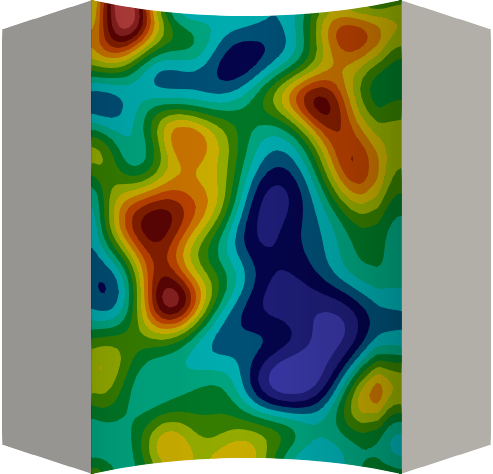
\includegraphics[width=\textwidth]{Chapter5/figures/spallation/E.0000}
  \end{subfigure}
  \begin{subfigure}{0.1\textwidth}
    \centering
    \caption*{$E/\underline{E}$}
    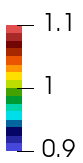
\includegraphics[width=\textwidth]{Chapter5/figures/spallation/colorbar_rf}
  \end{subfigure}
  \hspace{0.1\textwidth}
  \begin{subfigure}{0.25\textwidth}
    \centering
    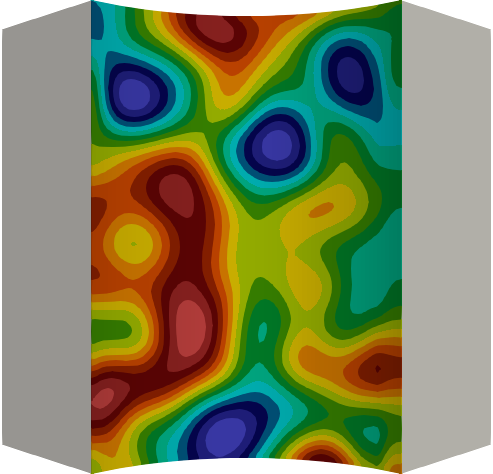
\includegraphics[width=\textwidth]{Chapter5/figures/spallation/Gc.0000}
  \end{subfigure}
  \begin{subfigure}{0.1\textwidth}
    \centering
    \caption*{$\Gc/\underline{\Gc}$}
    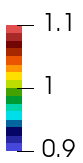
\includegraphics[width=\textwidth]{Chapter5/figures/spallation/colorbar_rf}
  \end{subfigure}
  \caption[Spatially varying Young's modulus and fracture toughness.]{Stationary marginally Gamma random fields normalized by their means: (a) Young's modulus; (b) fracture toughness. The coefficient variation is $0.3$.}
  \label{fig: Chapter5/spallation/random_fields}
\end{figure}
